\chapter{Architektury přístupových systémů}
Přístupové systémy jsou elektronické systémy řídící přístup uživatelů do omezených prostor v závislosti na jejich prokázané identitě. 
Běžně se s přístupovými systémy setkáváme zejména v kancelářních budovách, ale i nemocnicích, školách, úřadech apod.
Kromě řízení přístupu uživatelů do vybraných prostor přístupový systém umožňuje i zaznamenávat příchody a odchody uživatelů, tudíž je možné ho zároveň využít jako docházkový systém.
Tato kapitola osvětluje architekturu obecného přístupového systému jelikož se tato práce zabývá připojením senzorové sítě k infrastruktuře přístupového systému. 


Obrázek \ref{fig:Access control system architecture} zobrazuje typickou architekturu přístupového systému, kde identifikátor (ID Credential) představuje prvek umožňující identifikovat uživatele, např. RFID tag, otisk prstu nebo QR kód. 
Čtečka (Reader) slouží ke čtení dat z identifikátoru a v digitální podobě je odesílá k zařízení kontrolní panel (Control Panel).
Zámek dveří (Door Lock) řídí fyzický přístup uživatelů do omezených prostor. 
Kontrolní panel tvoří rozhraní mezi serverem řízení přístupu (Access Control Server) a páry čteček a zámků dveří.
kontrolní panely jsou obvykle připojeny k serveru řízení přístupu přes TCP/IP síť a páry čtečka a zámků dveří jsou obvykle připojeny ke kontrolnímu panelu přes RS485 síť. Databáze obsahuje všechna uživatelské ID.
Na serveru řízení přístupu je spuštěn Software (SW) spravující databázi a komunikující se všemi zařízeními typu Contril Panel.
Čtečka čte uživatelská ID z předložených identifikátorů a přeposílá je na kontrolní panel, který je dále přeposílá na server řízení přístupu. 
Access Control Software vyhledá obdržený uživatelský identifikátor v databázi a pokud je nalezen, pošle příkaz odpovídajícímu kontrolnímu panelu k přepnutí odpovídajícímu zámku dveří, čímž je uživateli udělen přístup do omezené oblasti \cite{accessControlSystem_eiprocus}.


\begin{figure}[!h]
    \centering
    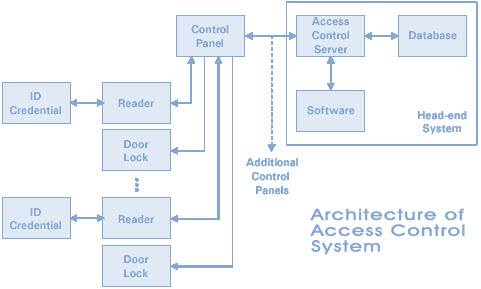
\includegraphics[width=1\textwidth]{Architetcture-of-Access-Control-System}
    \caption{Příklad architektury přístupového systému \cite{accessControlSystem_eiprocus}}
    \label{fig:Access control system architecture}
\end{figure}

